\chapter{Implementation}
This chapter is concerned with the implementation details of the individidual components introduced in Chapter \ref{chapter:4}. This includes the development of the Unity application responsible for producing a video stream from the front-facing camera of the Hololens, the development of the human detection and direction system, as well as the reactive control systems implemented on ARTA. Previous work in the PRL had utilized the Hololens camera to capture images that were then processed on an external computer, but where this project differs is that a video stream was required to be able to perform real-time object detection. As such, a large amount of time was spent at the very beginning of the project trying to produce a video stream, since the whole project depended on this form of visual input.

\begin{figure}[ht]
	\centering
	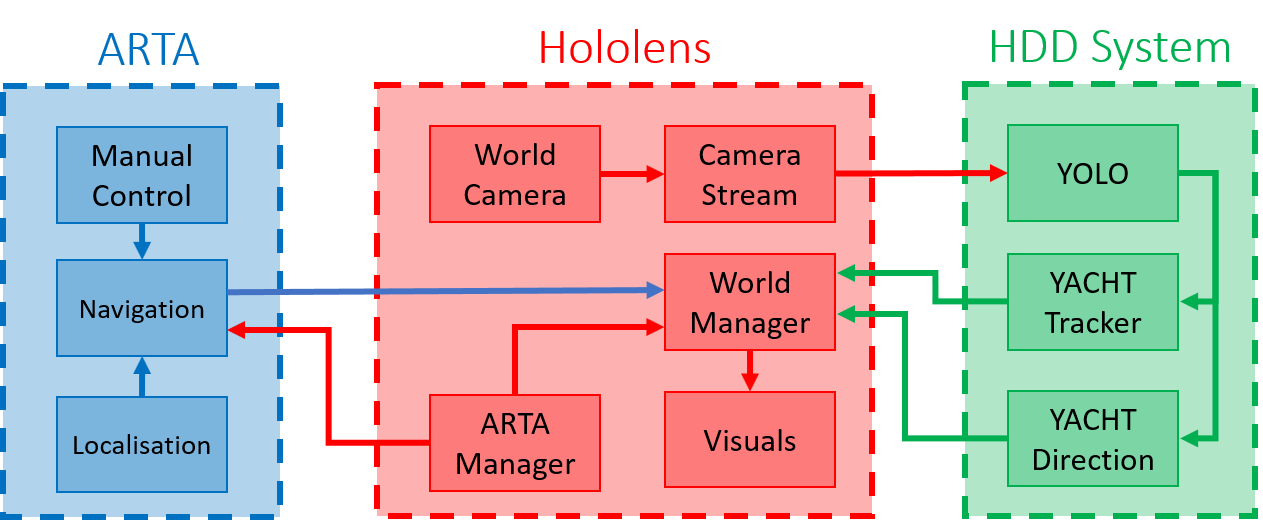
\includegraphics[width=1.0\linewidth]{img/chapter5_implementation/detailedSystemDiagram.png}
	\caption{System diagram detailing individual components}
	\label{fig:detailedHL}
\end{figure}

Figure \ref{fig:detailedHL} is a more detailed diagram of the high level system digram presented in Figure \ref{fig:simplifiedHL}. We show the communication between the three seperate devices, and how each node can be broken down into smaller nodes running specific computations. For the rest of this report, we represent ARTA, Hololens and HDD system components with the colours blue, red and green respectively.

%\section{Hololens Video Camera Stream}
%For this project to begin, it was absolutely essential to stream the front-facing camera on the Hololens to another PC. Once it had been proven that this was possible, work on the rest of the project could begin. As such, the first month of the project was spent comparing different camera streaming methods. As mentioned in Section \ref{sec:videoStreaming}, we briefly spent some time attempting to use the HoloLensForCV library from Microsoft. However, after speaking with several members of the PRL, it was decided the best method would be to use the Unity application approach as a base.


\section{Human Detection \& Direction System}
In order to be able to infer the direction people are walking in, it is necessary for the system to be able to detect humans. Only after detection is it possible to discern the motion of individuals, which can be achieved through object tracking and body pose estimation. This section is concerned with the implementation of the methods needed to perform the direction prediction, as well as how the system communicates between its nodes. Figure \ref{fig:detailedHDD} shows the breakdown of the HDD node into its seperate components. 

\begin{figure}[ht]
	\centering
	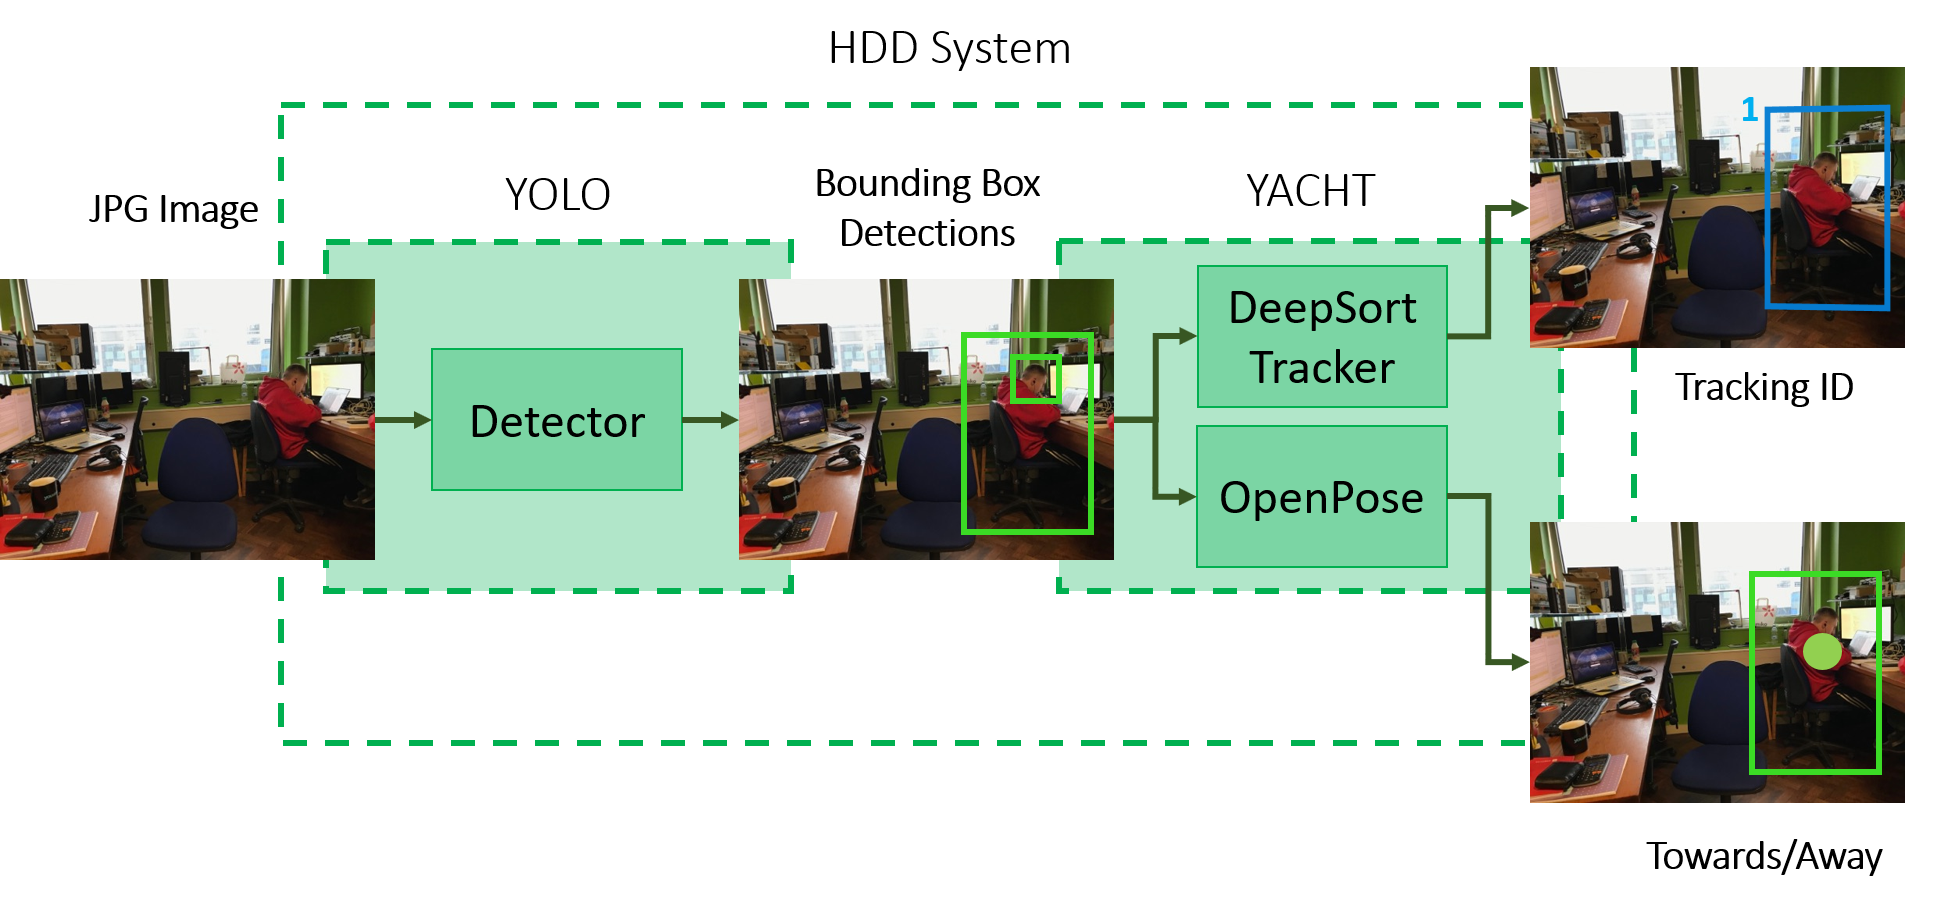
\includegraphics[width=1.0\linewidth]{img/chapter5_implementation/hddSystemDiagram.png}
	\caption{Individual nodes in HDD System}
	\label{fig:detailedHDD}
\end{figure}

We begin this section by listing the hardware requirements for the system. Due to the nature of the HDD, and its reliance on modern deep learning techniques, access to a modern GPU is essential. We refrain from trying to explain step-by-step how to setup the hardware and software, and instead point the reader in the direction of a Medium article\footnote{https://link.medium.com/xQ5w2FMXoX} which covers this topic.

\subsection{Hardware \& Software Dependencies}

\subsubsection{Hardware}
We implemented the HDD system on a desktop computer connected to the Imperial College network. Due to the real-time computer vision requirements of this project, the computer was chosen due to the GTX 1050Ti GPU with 4GB video RAM available on the system. The computer also had an Intel i7-2600 CPU and 8GB DDR3 RAM.

\subsubsection{Software}
We have refrained from posting every single Python dependency for the project. A complete listing is available in the appendix. The following software dependencies are required to run this project:
\begin{itemize}
	\item Ubuntu 16.04
	\item Python 2.7
	\item OpenCV 3.0
	\item ROS Kinetic
\end{itemize}

Due to the deep learning component of the project, the following software dependencies are essential:
\begin{itemize}
	\item Nvidia Graphics Drivers 
	\item CUDA 8.0 Toolkit
	\item cuDNN 6.0
	\item Darknet
	\item Tensorflow-GPU
	\item Caffe
\end{itemize}

\subsection{YOLO Object Detector}
As mentioned in Section \ref{sec:yolo}, we chose to use the YOLOv3-tiny architecture and trained it on the CrowdHuman dataset. We begin this section by introducing the reader to \textbf{Darknet}, the neural network framework YOLO is implemented on, and how we integrated it into ROS. We also briefly explain how the network detects objects, and compare YOLOv3-tiny with the more memory intensive YOLOv3. We then guide the reader through the training process, and the analysis we did to validate the human detection improvements compared to pre-trained models.

\subsubsection{Darknet}
Darknet\footnote{https://pjreddie.com/darknet/} is an open source neural network framework written in C and CUDA which supports both CPU and GPU computation \cite{darknet13}. The source code for the framework is freely available on Github, and can be used to train different neural network architectures in a manner similar to more conventional deep learning frameworks such as Tensorflow or Caffe.

\subsubsection{Darknet in ROS}
By definition, ROS is language-independent, although at the time of writing, three main libraries have been defined for ROS, making it possible to program ROS in Python, Lisp or C++. On the other hand, Darknet is implemented in C, due to the speed of compiled low-level languages in conjunction with CUDA. However, the Darknet framework is compiled into \textit{Shared Object (.so)} file, which is analogous to a Windows DLL. As such, it becomes possible to access the framework by writing wrappers around the compiled library file.

\paragraph{}Darknet has basic Python wrappers around the compiled library which convert Python datatypes into C and vice versa. However, the original wrappers for detection are written to run on images that are saved on disk. To integrate the framework into ROS, the node must be able to receive data from image topics with \code{CompressedImage} or raw \code{Image} messages.

\paragraph{}In Python, the JPG or PNG images received from the \code{CompressedImage} message can be converted to numpy arrays which store the RGB values. As such, we wrote Python wrappers for Darknet that would allow the framework to support images in the form of a numpy array as well as images saved on disk. This is done using the following code-snippet:

\begin{lstlisting}[language=Python]
# IMAGE: a C data structure used by Darknet
class IMAGE(Structure): 
	_fields_ = [("w", c_int),
				("h", c_int),
				("c", c_int),
				("data", POINTER(c_float))]
				
# Converts numpy array to Darknet IMAGE type
def nparray_to_image(img): 
	data = img.ctypes.data_as(POINTER(c_ubyte))
	image = ndarray_image(data, img.ctypes.shape, img.ctypes.strides)

	return image
\end{lstlisting}

Python wrappers were written for the detection and return of the image bounding box co-ordinates which are used in the rest of the HDD system. We also created ROS messages for the bounding box detections, which allows the Darknet YOLO node to communicate with other nodes in the HDD system. The full code listing can be found in the appendix \footnote{https://github.com/alaksana96/darknet-crowdhuman}\footnote{https://github.com/alaksana96/fyp\_yolo}.

\subsubsection{YOLO Detection Algorithm}
The YOLO algorithm divides an input image into an $S\times S$ grid. Each grid cell can predict one object, and a cell can predict a fixed number of bounding boxes $B$, which we visualize in Figure \ref{fig:yoloViz}. The predicted bounding box is chosen from the set of $B$ boxes with the highest box confidence score, which is a measure of how likely the box contains an object and how accurate the boundry box is. It also predicts the conditional class probability, which is the probability a detected object belongs to a certain class. 

\begin{figure}[ht]
	\begin{subfigure}[b]{.45\textwidth}
		\centering
		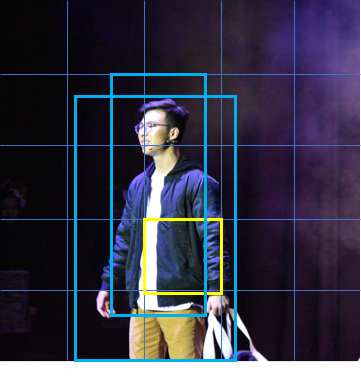
\includegraphics[width=1.0\linewidth]{img/chapter5_implementation/yoloAlgo1.png}
		\caption{A grid cell can make $B$ predictions, in this example $B=2$}
	\end{subfigure}%
	\hspace{\fill} 
	\begin{subfigure}[b]{.45\textwidth}
		\centering
		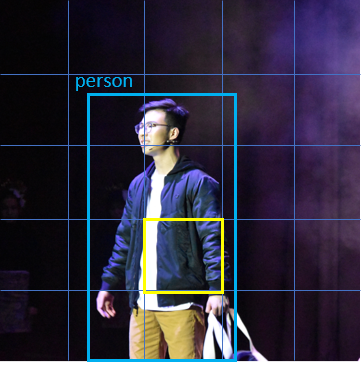
\includegraphics[width=1.0\linewidth]{img/chapter5_implementation/yoloAlgo.png}
		\caption{The bounding box with higher box confidence score is used}
	\end{subfigure}
	\vspace{-1\baselineskip}
	\begin{center}
		\caption{Visualization of YOLO person detection}
		\label{fig:yoloViz}
	\end{center}
	\vspace{-2\baselineskip}
\end{figure}


\subsubsection{YOLOv3 Tiny vs YOLOv3}
While testing out the different models, we noticed that the YOLOv3 model was consistently crashing and causing segmentation faults. On further investigation, we noticed that this was due to the network using up all 4GB of video memory available on the GPU. Looking at the architectures, YOLOv3, in comparison to its predecessors, YOLO and YOLOv2, is a much larger network which has 106 fully convolutional layers. This also reduces the framerates that can be achieved on video. As such, we decided to use YOLOv3 Tiny, a shallower variant of the network that is suitable for real-time image detection. Although the tiny version is not as accurate, it is much lighter on memory, using less than 1GB video RAM, making it a suitable choice for this project.

\subsubsection{Training YOLOv3 Tiny}
\paragraph{CrowdHuman} The CrowdHuman dataset \cite{Shao} is a benchmark dataset to better evaluate detectors in crowd scenarios. The most important features of the dataset are the size, the quality of the annotations and the diversity. Each image contains multiple people with varying degrees of occlusion, which allows for object detectors to better learn partial human repesentations. 

\begin{figure}[ht]
	\centering
	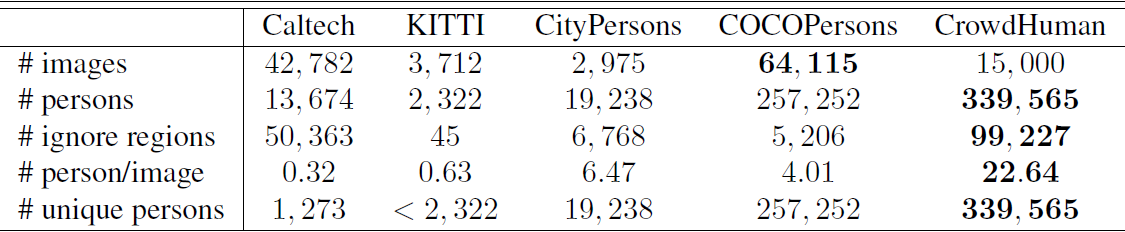
\includegraphics[width=1.0\linewidth]{img/chapter5_implementation/crowdHumanStats.png}
	\caption{A comparison of CrowdHuman to other person image datasets \cite{Shao}}
	\label{fig:crowdHumanStats}
\end{figure}

As can be seen from Figure \ref{fig:crowdHumanStats}, the dataset contains far more diversity in people. By examining the dataset, we can see that it contains people in a wide array of situations, at varying distances with different body poses.

\paragraph{Annotations} The CrowdHuman dataset provides its annotations in the \code{.odtg} format, which is a variant of JSON. Each line in the annotation file corresponds to a JSON containing the image ID and the bounding boxes. The annotations include boxes for the \textit{visible box}, \textit{full body box} and \textit{head box}. For the purposes of this training, we chose to use the full body and head boxes only. We wanted the detector be able to learn to predict occluded individuals, and we also wanted to experiment with head pose estimation. Each bounding box is annotated as such:

\paragraph{}\code{[x, y, width, height]} 

\paragraph{} Where \code{x,y} is the top-left corner of the bounding box. The \code{width} and \code{height} are also given in image co-ordinate pixels.

\paragraph{}On the other hand, to train YOLO on Darknet, the annotations must be given in a completely different format. The Darknet annotation format is as such:

\paragraph{}\code{<object-class> <x> <y> <width> <height>}

\paragraph{}Since Darknet accepts images of any size, it works with image units which are scaled relative to the size of the image. As such, all the values for the bounding boxes are between $0$ and $1$. Furthermore, the \code{x, y} values in the annotation are measured from the centre of the bounding box.  

\paragraph{Converting Annotations} To be able to use the CrowdHuman dataset as a training set for the YOLOv3-tiny model, we had to write several scripts that converted the annotations to the Darknet format. We have included these scripts in the Appendix should the reader wish to convert the dataset themselves\footnote{https://github.com/alaksana96/darknet-crowdhuman/blob/master/README.md}.

\paragraph{Training Parameters} Before beginning training, we set up the model configuration file to learn 2 classes, head and body, as well as to use batches of 32 divided into subdivision of 8 images. This means that only 8 images will be loaded into memory at a time, so as not to run out of GPU memory. However, this does mean the training process will take longer. We also reduce the size of the training images to $416\times 416$ pixels, to further reduce the GPU usage.

\begin{lstlisting}[language=Mymatlab,caption={Training parameters}]
	batch=32 %Training parameters for YOLO Tiny
	subdivisions=8
	width=416
	height=416
	channels=3
	momentum=0.9
	decay=0.0005
\end{lstlisting}

Resizing the input training images allows the algorithm to divide the image into a $S\times S$ grid. Generally, the larger the height and width, the better the predictions, since the image can be divided into more grid cells. This is a trade-off we had to make in order to be able to train the network on a mid-range GPU.

\paragraph{Training Process} We left the model to train overnight, creating backups of the weights every 1000 iterations. The following day, after reaching 30,000 iterations, we decided to stop training the network. This is because the average loss error and total loss had stopped decreasing for several hours, and was hovering around $29.134$. We reasoned that the network had reached a minima, and further training would be redundant, since it would just overfit the dataset. The final weights are available in the file \code{yolov3-tiny-crowdhuman.backup} .

\subsubsection{Evaluating Trained Model}


\subsubsection{ROS Node}

\paragraph{Visualization and FPS}

\paragraph{ROS Topic}


\subsection{YACHT Tracker}


\subsection{YACHT Direction}




%\section{Hololens Unity Application}
%
%\begin{figure}[ht]
%	\centering
%	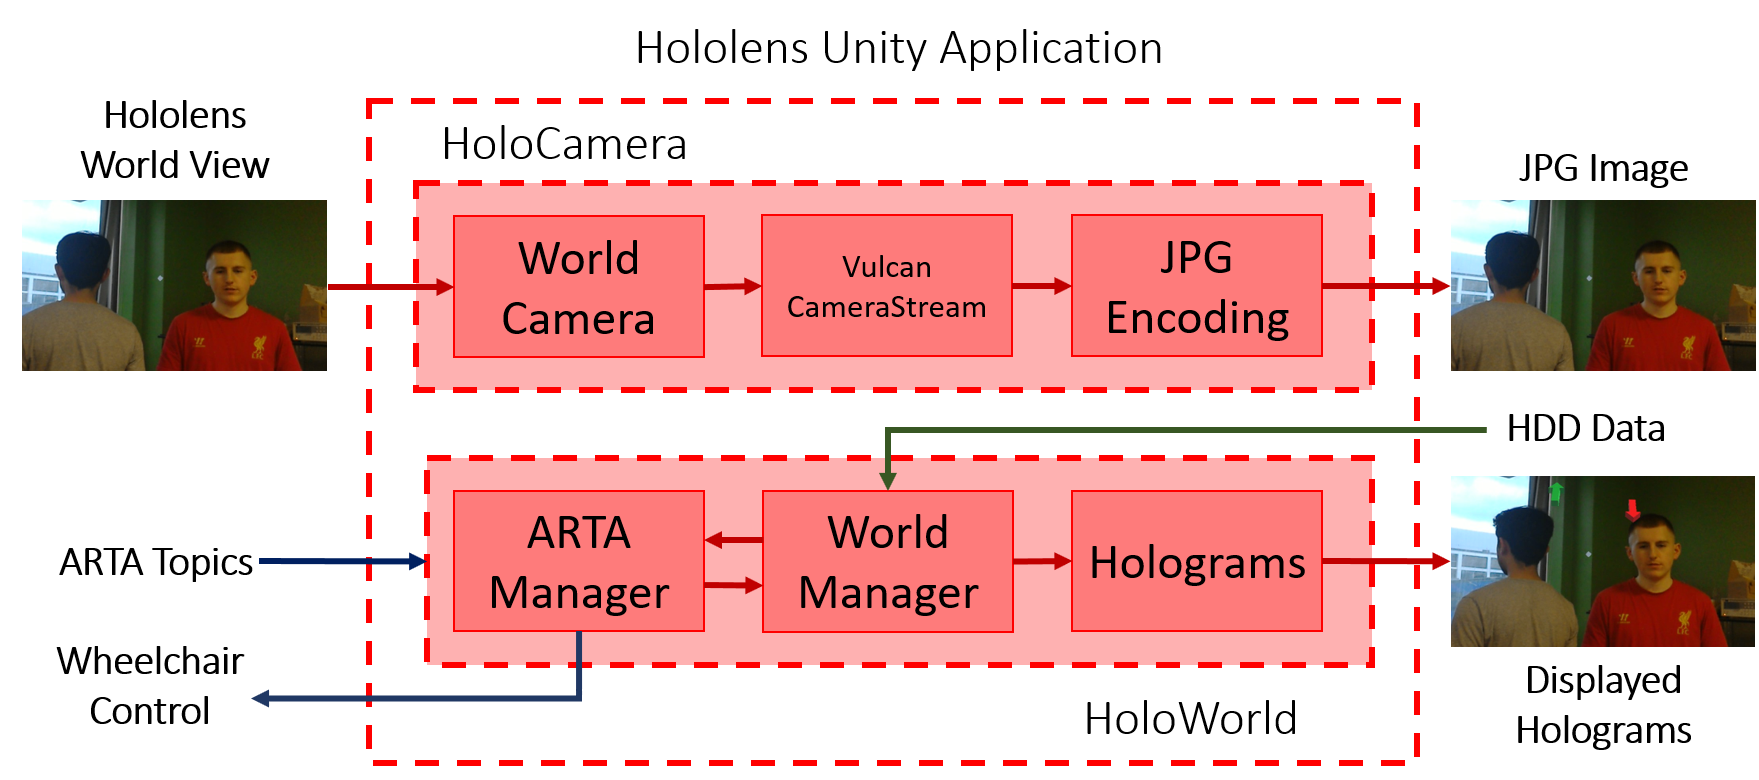
\includegraphics[width=1.0\linewidth]{img/chapter5_implementation/hololensSystemDiagram.png}
%	\caption{Unity application running on the Hololens}
%	\label{fig:detailedHololens}
%\end{figure}
